\section{System}
\label{sec:system}

In this paper we use the formulas from Kennedy's most recent definition of PSO~\cite{4223164}.
It can be easily extended to many versions of PSO.
This version of PSO includes a constricted position update rule, a personal best update and a star topology formed by a global best update.
The constricted position update rule is
\begin{subequations}
\label{eq:pso_alg}
\begin{equation}
\label{eq:up_vel}
\begin{aligned}
v_{ij}(k+1) = &  \chi [ v_{ij}(k) 
 + \phi^{P} u^{P}_{ij}(k) (x^{P}_{ij}(k) - x_{ij}(k))\\
 & + \phi^{G} u^{G}_{ij}(k) ( x^{G}_{ij}(k) - x_{ij}(k)) ],
\end{aligned}
\end{equation}
\begin{equation}
\label{eq:up_pos}
x_{ij}(k+1) = x_{ij}(k) + v_{ij}(k+1).
\end{equation}
\end{subequations}
$ x_{ij}(k) $ represents the position of particle $ i $ in dimension $ j $ at time $ k $.
$ v_{ij}(k) $ similarly represents the velocity of particle $ i $ in dimension $ j $ also at time $ k $.
$ x^{G}_{ij}(k) $ and $ x^{P}_{ij}(k) $ are global (actually topology) and personal best positions observed by the swarm and the particle respectively. 
$ u^{G}_{ij}(k) $ and $ u^{P}_{ij}(k) $ are independent random values drawn from $ [0,1] $.
$ \chi \in ( 0, 1 ) $, $ \phi^{P} $ and $ \phi^{G} $ are algorithm parameters.
The personal best update is
\begin{equation}
\label{eq:pb_up}
x_{i}^{P}(k) = \arg \max_{ x \in \{ x_{i}(k), x_{i}^{P}(k-1) \} } f(x).
\end{equation}
The global best update is
\begin{equation}
\label{eq:gb_up}
x_{i}^{G}(k) = \arg \max_{ x \in \{ x_{i}(k), x_{i}^{G}(k-1) \} } f(x).
\end{equation}
The share of the global best leads to a star topology in the swarm.

When particle $ i $ finds a position that is better than the current global best, it updates the global best and its personal best.
The swarm moves to a new global-best stagnation.
In this case, there is $ x_{i}(k) = x_{i}^{P}(k) = x_{i}^{G}(k) $ in the particle.
Equation \eqref{eq:up_vel} becomes
\begin{equation}
\label{eq:up_vel:leader}
v_{ij}(k+1) = \chi [ v_{ij}(k) 
 +( \phi^{P} u^{P}_{ij}(k) + \phi^{G} u^{G}_{ij}(k) ) (x^{G}_{ij}(k) - x_{ij}(k))  ].
\end{equation}
As the inertia of the previous velocity $ v_{ij}(k) $ will decay to zero,
the particle is attracted to $ x^{G}_{ij}(k) $ as $ \phi^{P} u^{P}_{ij}(k) + \phi^{G} u^{G}_{ij}(k) \geq 0 $.
This particle can be viewed as a leader of this swarm.
The topology is given in Figure \ref{fig:leader_follower}.
\begin{figure}[tbph]
\centering
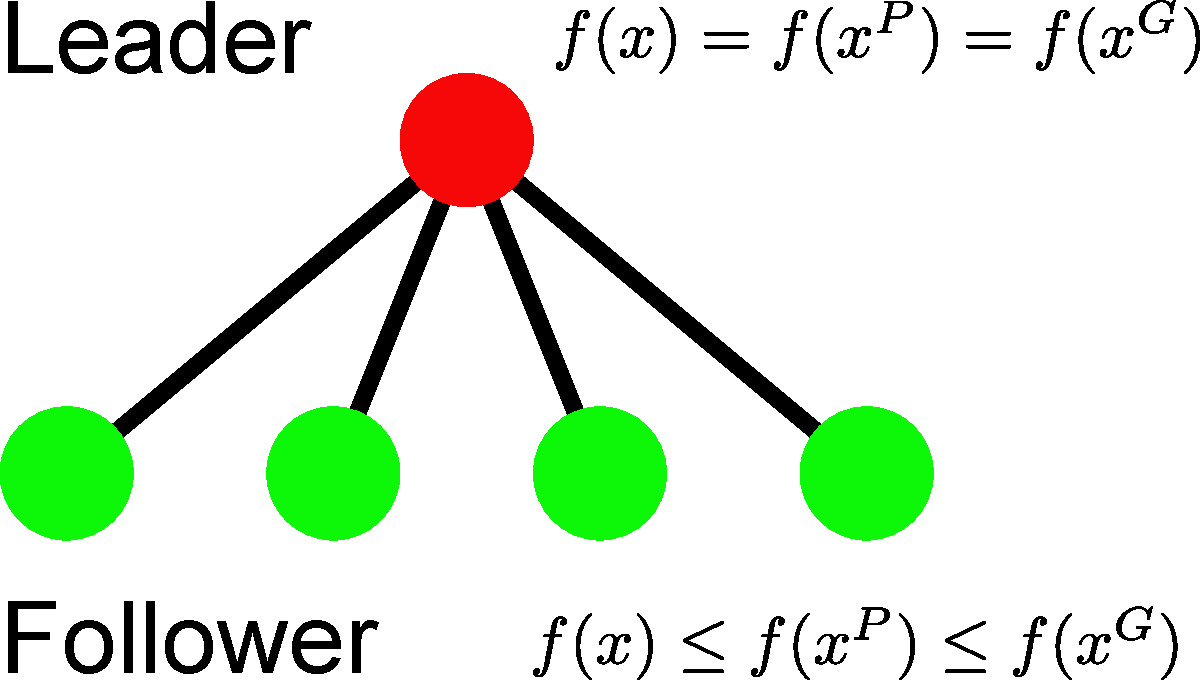
\includegraphics[width=0.5\linewidth]{./fig/leader_follower}
\caption{A leader-follower relationship.}
\label{fig:leader_follower}
\end{figure}

The star topology supports the leader competition among the particles.
The particle that finds a new global best becomes the leader of the swarm.
The other particles are the followers, which are attracted to the leader by the impact of the global best.
By Property \ref{prop:unconverge_neq_gb}, we know that a particle will never stop moving if the personal best and the global best are inconsistent.
Thus, we can view the movements of the followers are sampling in the solution space to solve the inconsistency between its own personal best and the global best.
The input to each particle from the topology of the swarm is only the global best.

\subsection{A feedback cascade model in a particle}

With the global best as the input, we model the behavior of a particle as a \emph{feedback cascade system}.
As shown in Figure \ref{fig:sys_flow}, this system is comprised of two components that form a feedback system structure.
These two components are 
the \emph{input-update component} for the personal best ($ x^{P}_{i}(k) $) and the global best ($ x^{G}_{i}(k) $), 
and the \emph{position-update component} for particle position ($ x_{i}(k+1) $), which depends on the inputs $ x^{G}_{i}(k) $ and $ x^{P}_{i}(k) $ as well as the last position $ x_{i}(k) $.

\begin{figure}
\centering
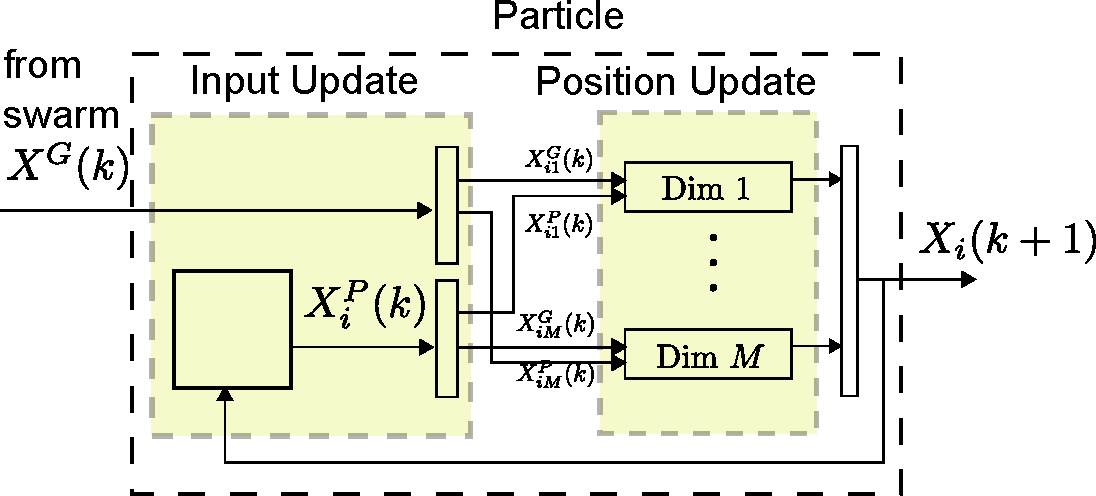
\includegraphics[width=0.85\linewidth]{./fig/sys_flow.pdf}
\caption{System structure of Particle.}
\label{fig:sys_flow}
\end{figure}

\begin{figure}
\centering
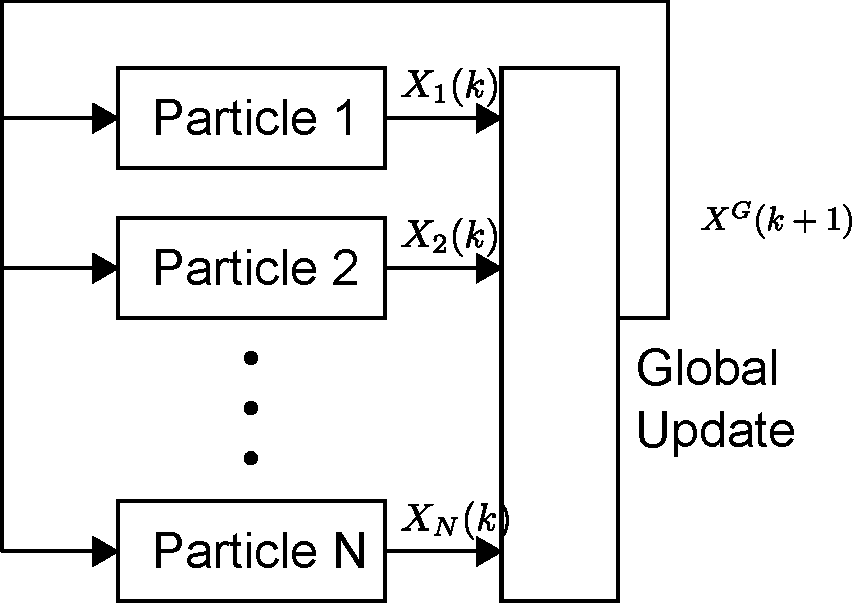
\includegraphics[width=0.6\linewidth]{./fig/pso_sys_flow.pdf}
\caption{System structure of Swarm}
\label{fig:pso_sys_flow}
\end{figure}

In the position-update component, the position at each dimension is updated by using the values from the $ x^{G}_{i}(k) $ and the $ x^{P}_{i}(k) $ in the corresponding dimension.
By Equation \eqref{eq:pso_alg}, we can decompose the position-update component into subcomponent in each dimension.
As shown in Figure \ref{fig:sys_flow}, the subcomponents in the position-update component form a parallel connection.
From \eqref{eq:pso_alg}, we can write a linear form of the position update component in one dimension.
\begin{equation}
\label{eq:pso_up_linalg_simp}
X(k+1) = A(k) X(k) + B(k) U(k)
\end{equation}
with
$ A(k) = \begin{bmatrix}
\chi & - \chi \phi^{G} u^{G}(k) - \chi \phi^{P} u^{P}(k)
\\ 
\chi & 1 - \chi \phi^{G} u^{G}(k) - \chi \phi^{P} u^{P}(k)
\end{bmatrix} $
and
$ B(k) = \begin{bmatrix}
\chi \phi^{G} u^{G}(k) & \chi \phi^{P} u^{P}(k)
\\ 
\chi \phi^{G} u^{G}(k) & \chi \phi^{P} u^{P}(k)
\end{bmatrix} $.
The system state is $ X(k) = [ v(k), x(k) - x^{R} ]^{T} $, and the system input is $ U(k) = [ x^{G}(k) - x^{R} , x^{P}(k) - x^{R} ]^{T} $.
\footnote{$ x^{R} $ means a reference point to the system.
When applying to the PSO, it can be a local optimum, a global optimum, or an estimated optimum.
We use it as a reference point to check the bounds.}
With a new $ x(k+1) $, the personal best update component will update the personal best $ x^{P}(k+1) $ that are fed into the position update component.

The input-update component consists of a \emph{global-best input} and a \emph{personal-best update}.
The personal best and global best are fed into the position-update component as input.
As in Figure \ref{fig:sys_flow}, the global-best input only takes the input from the swarm.
Thus the state to the reference point $ x^{R} $ is $  x^{G}(k) - x^{R} $.
The personal-best update compares the current $ x(k) $ with the $ x^{P}(k-1) $.
If  $ x_{i}(k) $ is better, the personal best is updated with it.
We can write the personal-best update as 
\begin{equation}
\label{eq:pso_input_up}
U = g^{PU}(V)
\end{equation}
with $ U = x^{P}(k) - x^{R} $ 
and $ V = x(k) - x^{R} $
from \eqref{eq:pb_up}. 

In Figure \ref{fig:sys_flow}, the position of a particle is modeled into a system with the input $ x^{G}(k) $ and the output $ x(k) $.
By using this model, we can have the system structure of a swarm in Figure \ref{fig:pso_sys_flow}.
There is a \emph{global update} that reads the states of all the particles and determine whether the global best should be updated.
The global best is fed back to all the particles for the next optimization iteration.

